\section{软件入门}
\subsection{软件安装与运行}
TBD

\subsection{界面概览}
\csciname 分为两个窗口:主窗口和视频窗口。

主窗口界面如图\ref{fmainwin}所示。

\begin{figure}[ht]
	\begin{center}
		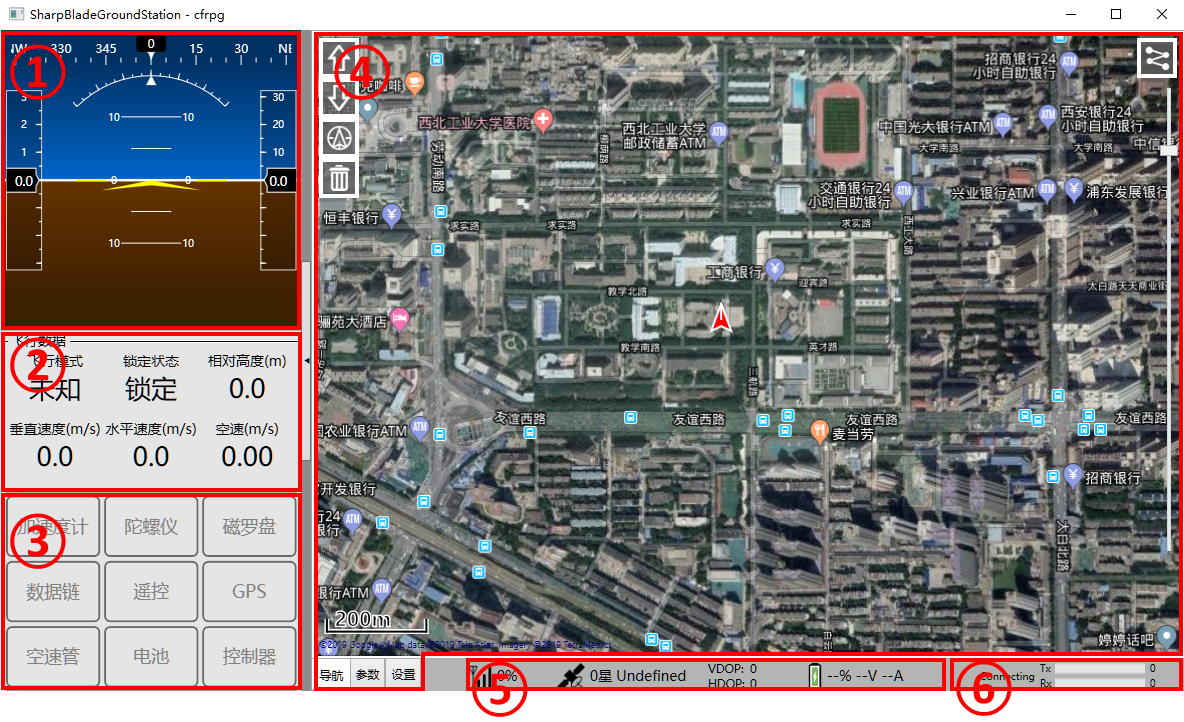
\includegraphics[width=\textwidth]{mainWindow.png}
		\caption{地面站主窗口}
		\label{fmainwin}
	\end{center}
\end{figure}

\begin{enumerate}[label=\arabic*.,topsep=0pt]
\setlength{\itemsep}{-2pt}
\item 主飞行显示器(PFD):显示无人机的姿态,高度及速度;
\item 飞行数据显示:显示飞行模式,锁定状态及部分飞行参数;
\item 告警灯:指示无人机飞控分系统异常;
\item 主功能窗口:地面站系统的主要功能部分,通过下方选项卡切换功能页面;
\item 无人机状态指示:显示信号强度,定位状态,供电状态等信息;
\item 连接状态指示器:控制无人机连接,显示当前连接状态。
\end{enumerate}

\clearpage

\subsubsection{主飞行显示器(PFD)}

\begin{figure}[ht]
	\begin{center}
		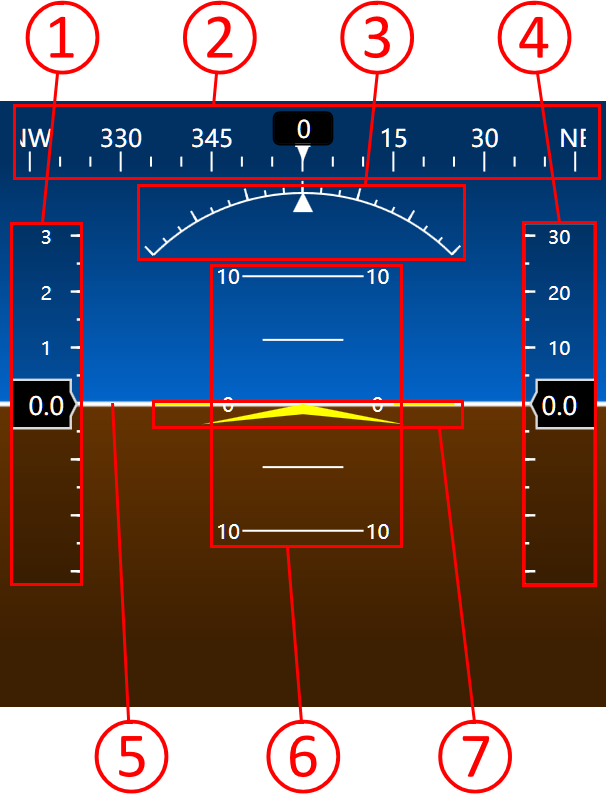
\includegraphics[width=0.6\textwidth]{pfd.png}
		\caption{主飞行显示器}
		\label{fpfd}
	\end{center}
\end{figure}

\begin{enumerate}[label=\arabic*.,topsep=0pt]
\setlength{\itemsep}{-2pt}
\item 速度标尺:显示当前的地速或空速,单位为m/s;
\item 航向标尺:显示当前的机头指向,一大格表示15\degree,一小格表示5\degree;
\item 滚转角指示:指示当前的滚转角,一大格表示15\degree,一小格表示5\degree;
\item 高度标尺:显示当前的海拔高度,单位为m;
\item 人工地平线;
\item 俯仰角标尺:一大格表示10\degree,一小格表示5\degree;
\item 飞机平面:代表飞机的水平面。
\end{enumerate}

\subsubsection{飞行数据显示}
飞行数据显示区以文字的形式显示飞机的飞行模式,锁定状态,相对高度,垂直速度,水平速度和空速。

\subsubsection{告警灯}
告警灯用于在飞控系统出现异常时提供警告,可能会表示为如图\ref{fwarn}的5种状态。各个状态的含义如表\ref{twarn}所示。
\begin{figure}[ht]
	\begin{center}
		
\includegraphics[width=0.6\textwidth]{warningLight.png}
		\caption{告警灯的五种状态}
		\label{fwarn}
	\end{center}
\end{figure}

\begin{table}[ht]
\centering
\caption{告警灯状态含义}
\label{twarn}
\begin{tabular}{ccl}
\toprule
\multicolumn{1}{c}{状态} & \multicolumn{1}{c}{颜色}   & \multicolumn{1}{c}{含义} \\ \midrule
熄灭 & 灰色 & 告警灯处于关闭状态 \\
提示 & 绿色 & 出现异常情况,但不影响飞行     \\
警告 & 黄色 & 出现异常,无法正常工作,可能影响飞行    \\
错误 & 红色 & 出现异常,无法工作,应停止飞行或降落    \\
严重 & 红色闪烁  & 出现严重问题,{\color{red}\textbf{应立即终止飞行}}   \\ \bottomrule
\end{tabular}
\end{table}

当告警灯点亮后通常不会自动熄灭,{\color{red}\textbf{在确认故障排除后} },左键点击告警灯可使告警灯熄灭。


\subsubsection{主功能窗口}
主功能窗口是\csciname 的主要交互区域,分为“导航”,“参数”,“设置”三个页面,鼠标点击下方的选项卡标签切换页面。

\subsubsection{无人机状态指示}
\begin{figure}[ht]
	\begin{center}
		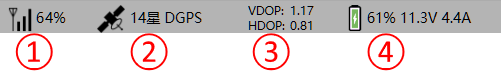
\includegraphics[width=0.7\textwidth]{status.png}
		\caption{无人机状态指示}
		\label{fstatus}
	\end{center}
\end{figure}
\begin{enumerate}[label=\arabic*.,topsep=0pt]
\setlength{\itemsep}{-2pt}
\item 数据链信号强度指示,以百分比显示数据链信号强度,当数据链不支持此功能时显示为0\%;
\item GPS状态指示:显示当前GPS卫星数与GPS定位状态;
\item GPS误差指示:显示GPS垂直误差和水平误差;
\item 电池状态指示:显示电池剩余电量百分比,电池电压和放电电流。
\end{enumerate}

\subsubsection{连接状态指示器}
\begin{figure}[ht]
	\begin{center}
		\includegraphics[width=0.5\textwidth]{commstate.png}
		\caption{连接状态指示}
		\label{fcomm}
	\end{center}
\end{figure}

连接状态指示器默认显示当前连接的状态。
如图\ref{fcomm}所示,左侧显示当前连接的方式(串口COM3)和使用的协议(MAVLink),右侧Rx,Tx条分别显示当前连接中接收数据的速率和发送数据的速率。

在没有与飞控连接的状态下,点击左侧部分可以打开如图\ref{fcommmenu}的连接选择菜单,选择使用串口连接飞控或进行日志回放。
\begin{figure}[ht]
	\begin{center}
		\includegraphics[width=0.5\textwidth]{commmenu.png}
		\caption{连接选择菜单}
		\label{fcomm}
	\end{center}
\end{figure}
\subsubsection{视频窗口}
TBD
\clearpage
\endinput
















